\documentclass[a4paper]{article}
\usepackage[a4paper,hmargin=3.5cm,vmargin=1.54cm,columnsep=2.02em]{geometry}
\usepackage{multirow}
\usepackage{amssymb}
\usepackage{amsmath}
\usepackage{booktabs}
%\usepackage{color}
\usepackage{prettyref}
\usepackage{indentfirst} 
\setlength{\parskip}{1.5ex plus 0.2ex minus 0.2ex}
\setlength{\parsep}{0ex} %段落间距
\renewcommand{\baselinestretch}{1.3}%设置行间距
%使用支持汉字的CJK包
\usepackage{CJK}
%调整列表行间距
\usepackage{paralist} 
\usepackage{graphicx}
\let\itemize\compactitem 
\let\enditemize\endcompactitem 
\let\enumerate\compactenum 
\let\endenumerate\endcompactenum 
\let\description\compactdesc 
\let\enddescription\endcompactdesc



\begin{CJK*}{UTF8}{song}


%这是文章的标题
\title{\CJKfamily{hei}{人工智能导论}\\{\large{第二次课程作业}\\Prof. Jianmin Li}}


\setlength{\parindent}{2em}%这是文章的作者
\author{马鸿鹏 2014012459}
\date{Submitted in \today}

%以上部分叫做"导言区",下面才开始写正文
\begin{document}


%先插入标题
\maketitle
%再插入目录
%\tableofcontents
\newpage
 \parindent 2em   %段首缩进
\section{Reflex Agent}
	

	\textbf{Solution}\\
	在第一个问题中,需要填写缺失的evaluationFunction, 这个函数的目的是为当前的状态打一个分数。\\
	我的思路是这样的,适合简单考虑的因素是食物,怪,当远离食物时施加一个惩罚,当远离怪的时候施加一个奖励
	,Pacman和这些物品之间的距离用曼哈顿距离来衡量,因为这个函数更符合Pacman和怪物在迷宫之中的移动
	\\
	公式如下:
	\begin{equation}
		ManhattanDistance(\vec{x}, \vec{y}) = \mathop{\sum}\limits_{i} abs(x_i - y_i)
	\end{equation}
	为了防止Pacman撞上怪物,当Pacman和怪物距离为0时增加一个超级大的惩罚,这是为了防止Pacman主动撞上怪物。
	其次对Pacman和怪物距离为1的时候加上一个小惩罚,因为这种情况很危险,ghost下一回合就可以吃掉Pacman。
	PS:这是一种极其简单的处理,在后面的Bonus题会在这个基础上有明显的改进。

	
	\begin{center}
        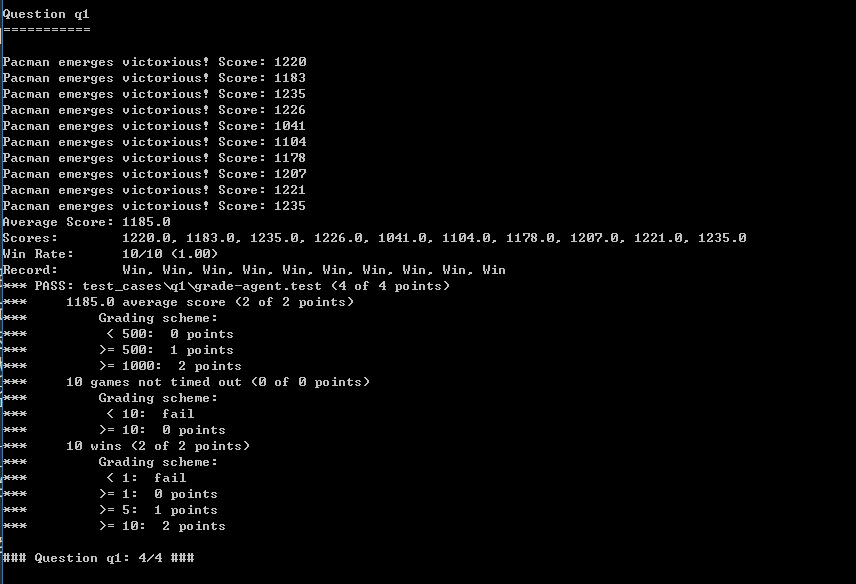
\includegraphics[width = 0.7\textwidth]{q1.png}\\
        Fig 1. Reflex Agent Result
    \end{center}

\section{MinimaxAgent, $\alpha-\beta$ pruning Agent}
  	\textbf{Solution}\\
  	这道题基本就是按照课上讲过的Minimax和$\alpha-\beta$实现一下,算法上面主要按照课上讲的内容实现即可。
  	出发点上是Pacman采取MaxMin策略,最大限度地提高在最糟糕情况下eval function的结果,而Ghost采取MinMax策略,
  	最大限度地惩罚Pacman,这个算法只有并不能确保给出最优解(Heuristic),这受限于使用的
  	evalFunction。\\
  	题外话,博弈论中的MaxMin Strategy 
  	\begin{equation}
  		\mathrm{Maxmin\ Strategy\ for\ player\ i} = arg\mathrm{max_{s_i}min_{s_{-i}}}u_{i}(s_1, s_2)
  	\end{equation}
  	其中 $\mathrm{s_{i}}$player i 采取的策略$\mathrm{s_{-i}}$是其他player采取的策略。
  	在有限步,两个player,零和游戏的纳什均衡点时Maxmin策略和Minmax策略相等,而本题中实现的算法并不能算是一个
  	确定能找到最优解(分数最高)策略。
\clearpage
\section{Expection Max Agent}
  	\textbf{Solution}\\
  	这种情况下考虑对手使用的策略服从某个分布,而在本题中则是平均分布(Ghost随机选择方向)。实际上相当于替换在
  	MiniMax算法中的Min-value函数,使之变成Ghost的行动在某一分布下的期望。\\
  	比较需要注意的是李老师在课上讲的对对手的预测并不是对手可能行动的平均,而是在一定分布下自己得分期望值,
  	这个算法最大化玩家得分的期望。


\section{better evaluation function}
  	\textbf{Solution}\\
  	\begin{center}
        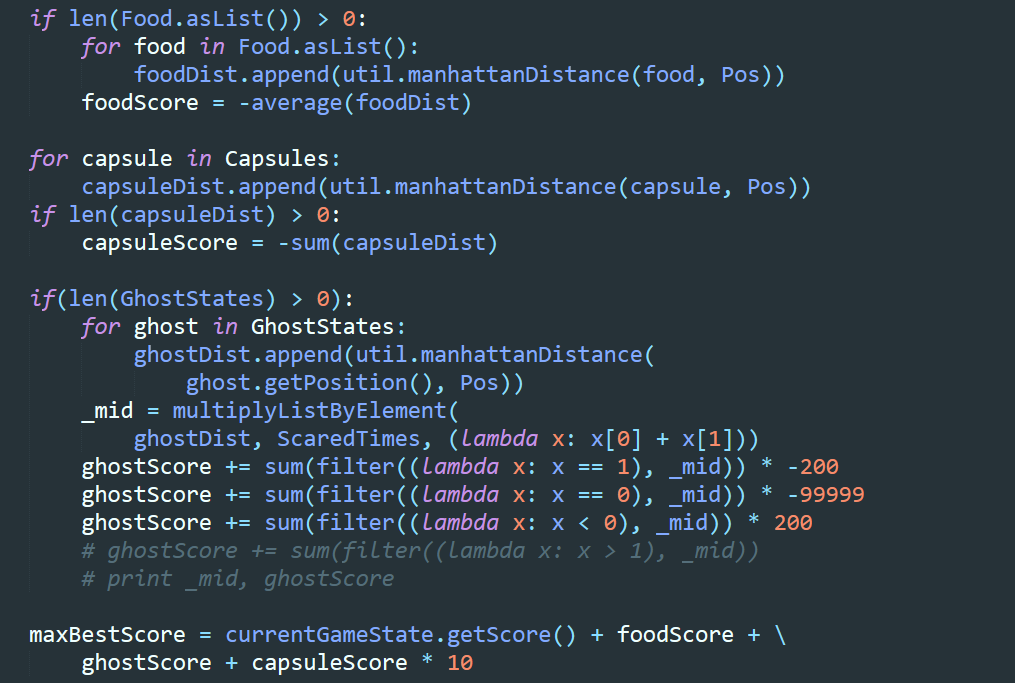
\includegraphics[width = 0.9\textwidth]{q5.png}\\
        Fig 2. Better Evalutaion Function Source Code
    \end{center}
  	我的改进主要在以下方向
  	\begin{itemize}
		\item 考虑食物的影响,离所有的食物距离均值(对总和做修正)越近越好
		\item 优先考虑虚弱Ghost的胶囊,它的权重是普通食物的10倍(这是一个人为指定的数字)
		\item 对正常的Ghost和快要恢复正常的Ghost采取回避策略,而对虚弱Ghost采取优先击杀的策略
	\end{itemize}
	最后的Evaluation Function
	\begin{center}
		\begin{equation}
			\mathrm{Evaluation\ Function} = \mathrm{Current\ State\ Score + Average(Food\ Distance)}\\
			\mathrm{ + Sum(Capsule\ Distance) * weight + Ghost\ Score}
		\end{equation}
	\end{center}
	这个函数很多改进的方向,比如对参数的调优,考虑墙壁的影响等等
\end{CJK*}
\end{document}\documentclass[a4paper]{article}

